%% LaTeX-Beamer template for KIT design
%% by Erik Burger, Christian Hammer
%% title picture by Klaus Krogmann
%%
%% version 2.1
%%
%% mostly compatible to KIT corporate design v2.0
%% http://intranet.kit.edu/gestaltungsrichtlinien.php
%%
%% Problems, bugs and comments to
%% burger@kit.edu

\documentclass[18pt]{beamer}

%% SLIDE FORMAT

% use 'beamerthemekit' for standard 4:3 ratio
% for widescreen slides (16:9), use 'beamerthemekitwide'

\usepackage{templates/beamerthemekit}
% \usepackage{templates/beamerthemekitwide}

%% TITLE PICTURE

% if a custom picture is to be used on the title page, copy it into the 'logos'
% directory, in the line below, replace 'mypicture' with the 
% filename (without extension) and uncomment the following line
% (picture proportions: 63 : 20 for standard, 169 : 40 for wide
% *.eps format if you use latex+dvips+ps2pdf, 
% *.jpg/*.png/*.pdf if you use pdflatex)

\titleimage{title}

%% TITLE LOGO

% for a custom logo on the front page, copy your file into the 'logos'
% directory, insert the filename in the line below and uncomment it

%\titlelogo{mylogo}

% (*.eps format if you use latex+dvips+ps2pdf,
% *.jpg/*.png/*.pdf if you use pdflatex)

%% TikZ INTEGRATION

% use these packages for PCM symbols and UML classes
% \usepackage{templates/tikzkit}
% \usepackage{templates/tikzuml}

% the presentation starts here

\title[Specification presentation]{Dynamic scheduler for scientific simulations}
\subtitle{Final presentation}
\author{Kai Bittner, Ard Kastrati, Fabio Broghammer, Jan Ellmers, David Krenz, Benjamin-Philip Roth}

\institute{Steinbuch Centre for Computing - SCC}

% Bibliography

\usepackage[citestyle=authoryear,bibstyle=numeric,hyperref,backend=biber]{biblatex}
\addbibresource{templates/example.bib}
\bibhang1em
\usepackage{graphicx}
\usepackage{tikz}
\usetikzlibrary{shapes}
\begin{document}

% change the following line to "ngerman" for German style date and logos
\selectlanguage{english}

%title page
\begin{frame}
\titlepage
\end{frame}

%table of contents
\begin{frame}{Outline}
\tableofcontents
\end{frame}


\section{Overview}
\begin{frame}{Overview}

\centerline{\includegraphics[scale=0.43]{images/overview}}
\end{frame}

\section{Scheduler}

	\begin{frame}{Master-Worker}
		\centerline{\includegraphics[scale=0.5]{images/master}}
	\end{frame}
	\begin{frame}{Task Stealing}
		\centerline{\includegraphics[scale=0.5]{images/taskstealing}}
	\end{frame}

	\begin{frame}{Scheduling strategies}
	\begin{minipage}[]{.7\textwidth}%
			\begin{itemize}
		\item<1-> non-statistical
		\begin{itemize}
			\item First In-First out (FIFO)
			\item Last In-Last out (LIFO)
		\end{itemize}
		\item<2-> statistical
		\begin{itemize}
			\item Shortest job first (SJF)
			\item Longest job first (LJF)
		\end{itemize}
		\item<3-> standardized interface - simple to include new strategies
		\end{itemize}
\end{minipage}%
\begin{minipage}[]{.3\textwidth}%
  \vspace{-\ht\strutbox}\includegraphics[width=\textwidth]{images/fifo}%
\end{minipage}		
		
	\end{frame}
	\begin{frame}{Scheduling strategies: Master-Worker vs. Task stealing}
		\begin{itemize}
			\item<1-> Master-Worker
				\begin{itemize}
					\item fast standard c++ implementation
					\item dynamic size
					\item easy to switch between scheduling strategies at runtime	
				\end{itemize}
			
			\item<2-> Task stealing
					\begin{itemize}
						\item custom implementation inside a MPI-Window
					\end{itemize}
			
		\end{itemize}
	\end{frame}


\section{Database}
%\subsection{stuff}

\subsection{database}

	\begin{frame}{What? - Metadata of a task}
		\begin{itemize}
		\item Identifier(ID)
		\item Timestamp of an event
		\item Event itself
		\item Mode
		\item Parent
		\item Rank
		%\item Intercommunication timestamp
		\item Number of parameters
		\item Parameters themselves
		\end{itemize}
	\end{frame}
	
	\begin{frame}{How? - Structure}
		\begin{itemize}
		\item Stored data in 2 seperated files
		\item Bookkeeping: listed data of previous slide
		\item Statistics: parameters and runtime of a task
		\item Files are accessable for visualizer
		\end{itemize}
	\end{frame}
\subsubsection{handling}
	\begin{frame}{DatabaseHandler}
	\includegraphics[width=0.3\textwidth]{images/databasehandler.png}
	\begin{itemize}
		\item Provides methods for data parsing
		\item Passes data through
		
	\end{itemize}
	\end{frame}
	
	\begin{frame}{DatabaseServer}
	\includegraphics[width=1.0\textwidth]{images/Zeichnung6.png}
	\end{frame}
	
	\begin{frame}{Database - DataMining}
	\centering
	\includegraphics[width=0.55\textwidth]{images/datamining_flow.png}
	\end{frame}


	\begin{frame}{Introduction}
		\begin{itemize}
			\pause
			\item Easy usage of MOAB Workload Manager and Dynamic Scheduler
			\pause
			\item Generate shell scripts for MOAB Workload Manager 
			\begin{itemize}
				\pause
				\item  send script via SSH to the bwUniCluster
			\end{itemize}
			\pause
			\item Visualization
			
		\end{itemize}
	\end{frame}
	
	\begin{frame}{Architecture}
		\begin{itemize}
	\pause
			\item Model-View-Presenter
			\begin{itemize}
				\pause
				\item FXML to describe the UI
				\pause
				\item Java code for application logic
			\end{itemize}
	        
				\includegraphics[width=300px, height=100px]{images/mvp.png}
		\end{itemize}
	\end{frame}
	
	
%	\subsection{Design}
%	\begin{frame}{Architecture (Design)}
%		\includegraphics[width=300px, height=210px]{images/GUIDesign.png}
%	\end{frame}
	

	\begin{frame}{SSH-Connection}
		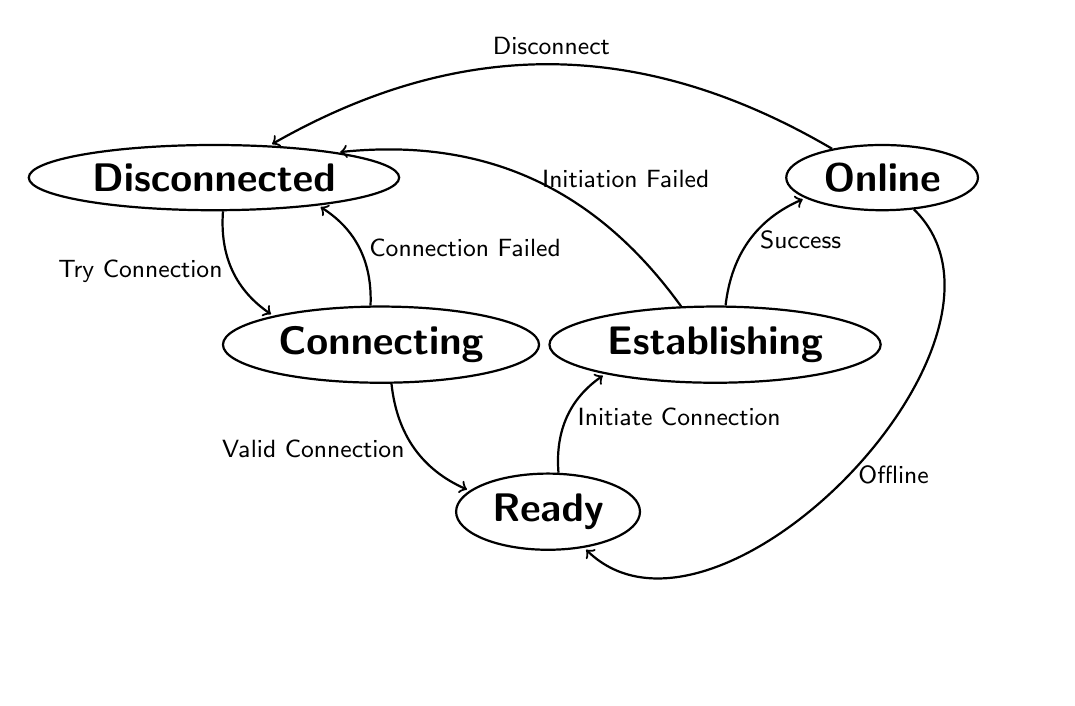
\begin{tikzpicture}[->,shorten >=1pt,auto,node distance=3cm,thick,main node/.style={ ellipse,draw,font=\sffamily\Large\bfseries}]
 
  \node[main node] (1) {Disconnected};
  \node[main node] (2) [below right of=1]{Connecting};
  \node[main node] (3) [below right of=2] {Ready};
  \node[main node] (4) [above right of=3] {Establishing};
  \node[main node] (5) [above right of=4] {Online};

  \path[every node/.style={font=\sffamily\small}]
    (1) edge [bend right] node[left] {Try Connection} (2)
        
    (2) edge [bend right] node[right] {Connection Failed} (1)
        edge [bend right] node[left] {Valid Connection} (3)
    (3) edge [bend left] node[right] {Initiate Connection} (4)
    		
    (4) edge [bend right] node[right] {Initiation Failed} (1)
       	edge [bend left] node[right] {Success} (5)
    (5)  edge [bend right] node[above] {Disconnect} (1)
         edge [bend left=90] node[right] {Offline} (3);
	\end{tikzpicture}
	\end{frame}
	
	\begin{frame}{Script Generator}
	\begin{itemize}
		\pause
		\item Shell script generator for MOAB Workload Manager:
		
		\begin{itemize}
			\pause
			\item parse msub command
			
			\pause			
			\item specify the directory in server using lazy tree 
			 
			\pause
			\item parse mpirun command
			
			\pause
			\item parse parameters of the dynamic scheduler
		\end{itemize}
			\end{itemize}
	\end{frame}
	
	
	
	\begin{frame}{Script Structure}
		
		\begin{block}{run\_scheduler.sh}
		        \#\#\#\# MOAB commands
		        \newline
		        \newline
				\#MSUB  -q develop\\
				\#MSUB  -l nodes=22:ppn=22\\
				\#MSUB  -l walltime=1000\\
				\#MSUB  -M uxdok@student.kit.edu
				\newline
				\newline
        				\#\#\#\# Directory
				\newline
				\newline
				cd ./Documents
				\newline
				\newline
        				\#\#\#\# MPI commands
        			\newline
        			\newline
				mpirun -np 4 ./myExec -design master-worker -strategy fifo
			
		\end{block}
	\end{frame}
	
	
\begin{frame}
	\begin{center}
			\huge{\textbf{Live Demo}}
	\end{center}		
\end{frame}
\section{Statistics}
\begin{frame}{Statistics}
	\begin{itemize}
		\item approx. 300 commits during 143 days
		\item average 2.1 commits per day
		\item 4000 lines of Java code
		\item 3500 lines of C++ / C code
		\item TeX, Makefile and XML
	\end{itemize}
\end{frame}
\section{Experience}
\begin{frame}{Experience}
	\begin{itemize}
		\item it is hard to understand whats the actual problem
		\item bigger changes during the implementation are hard to handle
		\item how fast you learn a unknown language (C++)
	\end{itemize}
\end{frame}
\begin{frame}
	\begin{center}
			\huge{\textbf{End}}
	\end{center}		
\end{frame}
\end{document}
